\chapter{TikZ and Drawing in \LaTeX}

\section{What is TikZ?}

TikZ is a powerful package for creating graphics programmatically within LaTeX. It stands for “TikZ ist kein Zeichenprogramm” (TikZ is not a drawing program), and is used for:

\begin{itemize}
	\item Diagrams
	\item Flowcharts
	\item Geometrical figures
	\item Graphs and trees
\end{itemize}

\section{Loading the Package}

Add the following in your preamble:

\begin{verbatim}
	\usepackage{tikz}
\end{verbatim}

\section{Basic Drawing Syntax}

Use the \texttt{tikzpicture} environment to begin drawing:

\begin{verbatim}
	\begin{tikzpicture}
		\draw (0,0) -- (2,0);        % a horizontal line
		\draw (0,0) -- (0,2);        % a vertical line
	\end{tikzpicture}
\end{verbatim}

\begin{center}
	\begin{tikzpicture}
		\draw (0,0) -- (2,0);
		\draw (0,0) -- (0,2);
	\end{tikzpicture}
\end{center}

\section{Drawing Shapes}

TikZ allows you to draw:

\begin{itemize}
	\item Lines: \verb|\draw (0,0) -- (2,2);|
	\item Rectangles: \verb|\draw (0,0) rectangle (2,1);|
	\item Circles: \verb|\draw (1,1) circle (0.5);|
\end{itemize}

\begin{example}[Circle and Rectangle]
	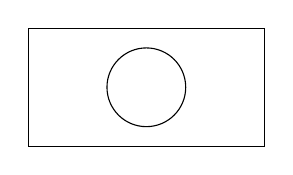
\begin{tikzpicture}
		\draw (0,0) rectangle (3,1.5);
		\draw (1.5,0.75) circle (0.5);
	\end{tikzpicture}
\end{example}

\section{Adding Text Labels}

Use \verb|\node| to place text at a position:

\begin{verbatim}
	\node at (0,0) {Origin};
\end{verbatim}

\begin{center}
	\begin{tikzpicture}
		\draw[->] (0,0) -- (2,0) node[right] {$x$};
		\draw[->] (0,0) -- (0,2) node[above] {$y$};
		\node at (0,0) [below left] {$(0,0)$};
	\end{tikzpicture}
\end{center}

\section{Arrows and Styles}

TikZ provides arrows and line styles:

\begin{itemize}
	\item \verb|->|: Arrow from first to second point
	\item \verb|dashed|, \verb|dotted|: Line styles
	\item \verb|thick|, \verb|ultra thick|: Line weights
\end{itemize}

\begin{example}
	\begin{tikzpicture}
		\draw[->, thick] (0,0) -- (2,1);
		\draw[dashed] (0,0) -- (1,-1);
	\end{tikzpicture}
\end{example}

\section{Simple Tree Structure}

\begin{verbatim}
	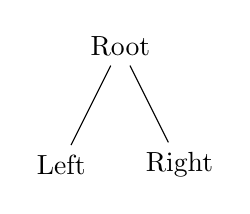
\begin{tikzpicture}
		\node {Root}
		child { node {Left} }
		child { node {Right} };
	\end{tikzpicture}
\end{verbatim}

\begin{center}
	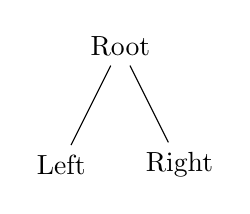
\begin{tikzpicture}
		\node {Root}
		child { node {Left} }
		child { node {Right} };
	\end{tikzpicture}
\end{center}

\section{Coordinate Grid (Optional)}

You can show a grid for layout:

\begin{verbatim}
	\draw[step=1cm, gray, very thin] (0,0) grid (4,4);
\end{verbatim}

\section{Packages for Graphs}

For more advanced graph theory or plots, consider:

\begin{itemize}
	\item \texttt{pgfplots}
	\item \texttt{circuitikz}
	\item \texttt{tkz-graph}
\end{itemize}

\section{Exercise}

\begin{exercise}
	Draw a simple diagram using TikZ:
	\begin{itemize}
		\item A coordinate axis with labels
		\item A rectangle with a circle inside it
		\item A labeled arrow from point $A$ to $B$
		\item A simple binary tree
	\end{itemize}
\end{exercise}
